\section{Continuous Integration}
Projektet er sat op, så der benyttes continuous integration, så projektet bliver bygget på en ekstern server, hver gang der bliver tilføjet en ændring til projektet via git. CI er blevet brugt for at undgå integrations problemer, der kan opstå, når flere gruppemedlemmer arbejder samtidig på samme projekt.
I forbindelse med at projektet bliver bygget på CI-serveren bliver de projektets test samtidig kørt.

TeamCity blev anvendt som CI-server, hvor der blev opsat et  projekt, der blev sat til at pege på gruppens github-repository. Projektet blev sat op til, at hver gang der blev "pushed" til reopistoriet skulle TeamCity kører to "Build Steps". I første step blev projektet bygget ved brug af MSBuild Tools 2015. Hvis det første skridt gik godt blev anden step udført, der bestod i at køre Test-projektets NUnit-tests. Testene blev kørt ved brug af en NUnit.ConsoleRunner, der var blevet installeret som en NuGet-Package i projektet.  
CI-projeket blev også tilknyttet en dotCover-test, der skulle fungere som et pejlemærke for, hvor stor en del af projektet testene dækker. Da der ikke var nogen specielle krav til Coverage-analysen blev JetBrains standard dotCover fil benyttet.

Nedenunder kan et eksempel af et build ses. 
\begin{figure}[ht!]
	\centering
	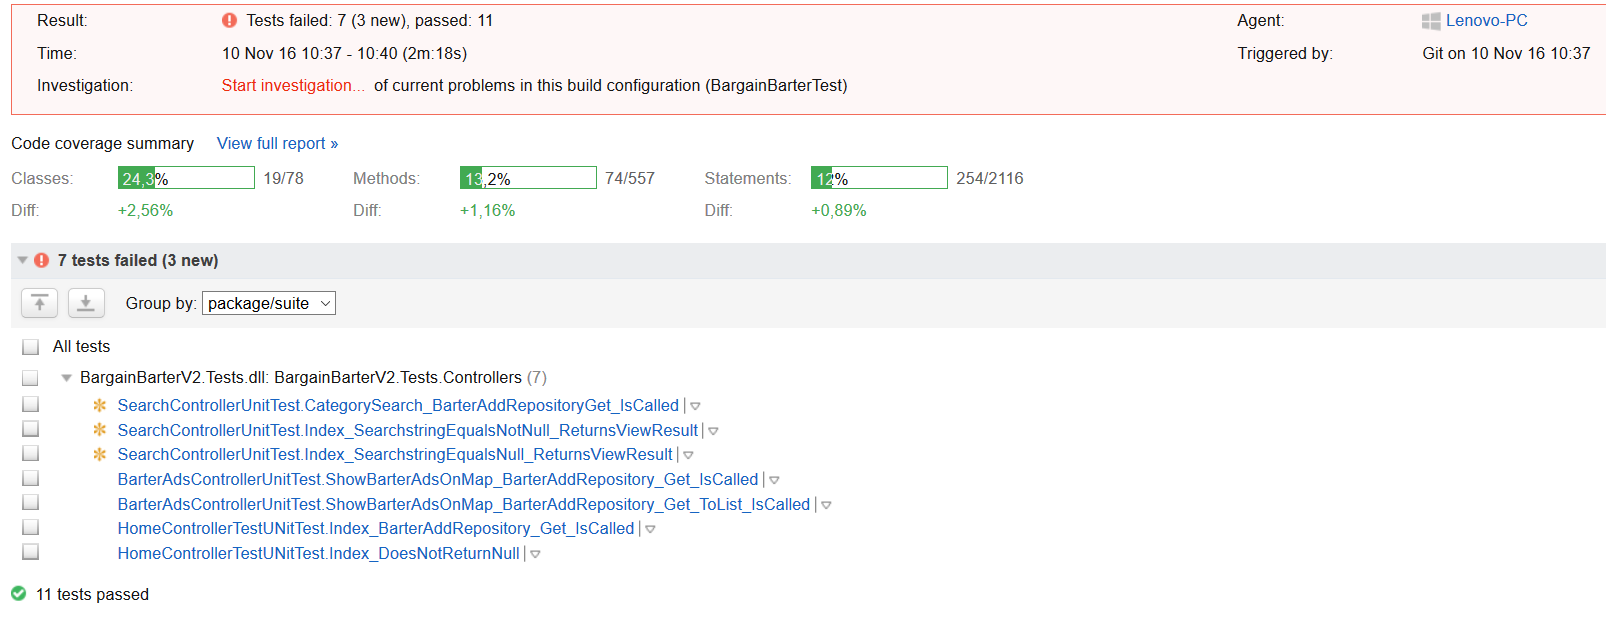
\includegraphics[width=120mm]{figures/TeamCityTest.png}
\end{figure}
